\documentclass[tikz,border=4pt]{standalone}
\usepackage[utf8]{inputenc}
\usepackage[T1]{fontenc}
\usepackage{graphicx}
\usepackage{amsmath,amssymb}
\usepackage{tikz}
\usetikzlibrary{arrows.meta,positioning,shapes.geometric,fit,calc,backgrounds,decorations.pathreplacing}
\definecolor{granate}{RGB}{138,0,0}
\definecolor{pizarra}{RGB}{43,58,85}
\definecolor{verdee}{RGB}{46,125,50}
\definecolor{ambar}{RGB}{242,169,0}
\definecolor{grisb}{RGB}{158,158,158}
\definecolor{grisc}{RGB}{238,238,236}
\definecolor{celeste}{RGB}{42,120,214}
\tikzset{
  bloque/.style={draw=pizarra,fill=white,rounded corners=3pt,thick,align=center,font=\sffamily\small,inner sep=5pt,minimum height=1.0cm},
  alcance/.style={bloque,fill=granate!10,draw=granate,very thick},
  fuera/.style={bloque,fill=grisc,draw=grisb,dashed,text=black!55},
  flecha/.style={-{Stealth[length=2.6mm]},thick,draw=pizarra},
  flechaf/.style={-{Stealth[length=2.6mm]},thick,draw=grisb,dashed},
  etiq/.style={font=\sffamily\scriptsize,text=pizarra,align=center}
}

\newif\ifresaltar\resaltarfalse
\begin{document}
\begin{tikzpicture}[node distance=9mm and 14mm]
\ifresaltar\tikzset{b/.style=alcance,f/.style=fuera}\else\tikzset{b/.style=bloque,f/.style=bloque}\fi
\node[b] (cont) {\textbf{Contrato de escenarios}\\ y 5 métricas\\{\scriptsize YAML versionado}};
\node[b,below=of cont] (cad) {\textbf{Biblioteca CAD}\\ celda de \emph{machine tending}\\{\scriptsize mesa, CNC, prensa, carro\ldots}};
\node[b,right=of cont,xshift=6mm] (gen) {\textbf{Generador}\\ \textbf{de escenarios}\\{\scriptsize 100 escenas + 19 variantes}};
\node[b,right=of gen,minimum width=4.4cm,minimum height=3.2cm,label={[etiq,yshift=1pt]above:Simulación de entrenamiento}] (env)
  {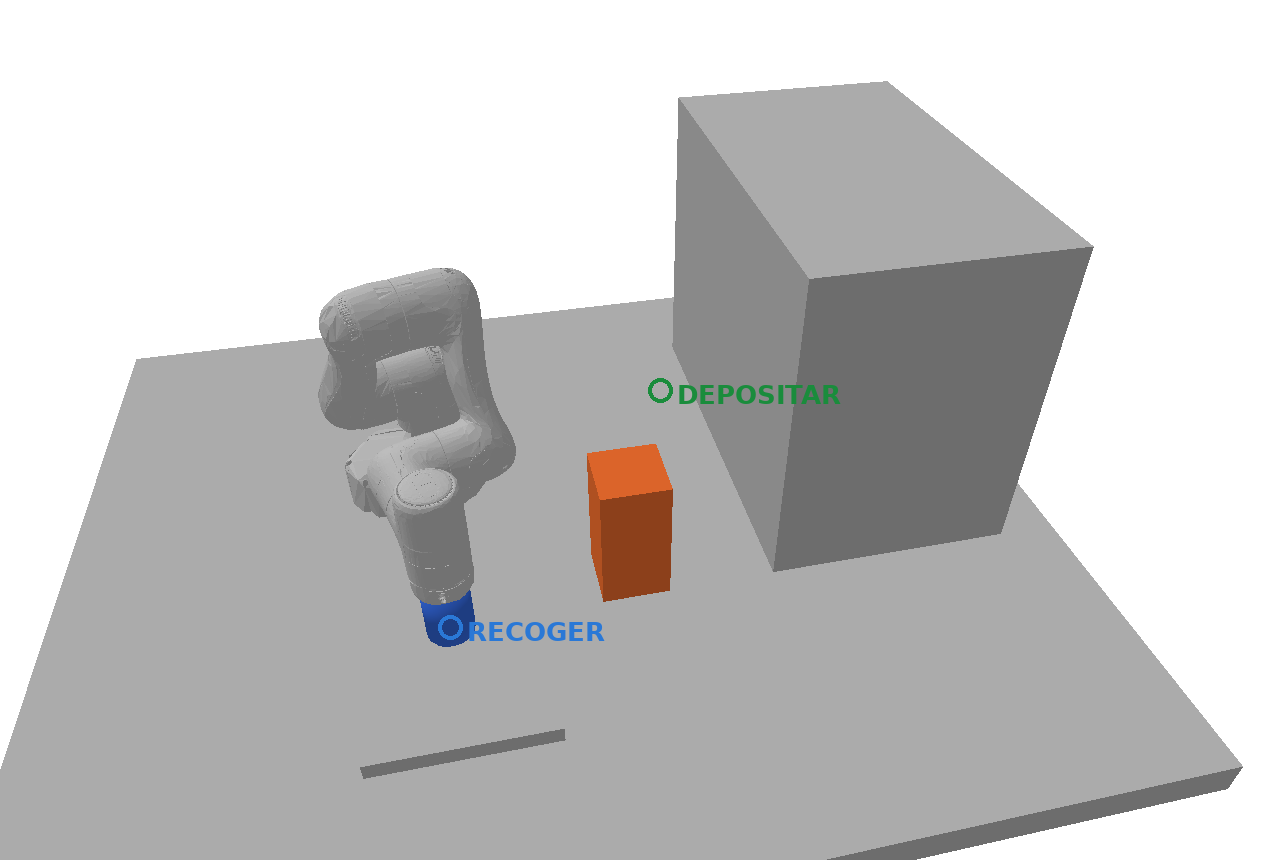
\includegraphics[width=4.0cm]{../img/escena_2.png}\\[1pt]\textbf{Entorno Gymnasium + PyBullet}\\{\scriptsize DOBOT Magician E6 · $\Delta t=30$ ms}};
\node[b,right=of env,minimum width=3.2cm] (sac) {\textbf{Agente SAC}\\ actor $\pi_\phi$ + 2 críticos\\[-1pt]{\scriptsize 43 observaciones $\to$ $\Delta q\in\mathbb{R}^6$}};
\node[b,below=of sac] (pc) {\textbf{PC de entrenamiento}\\ GPU GTX 1080 · 8 núcleos\\{\scriptsize PyTorch + Stable-Baselines3}};
\node[b,below=of env,yshift=-14mm,minimum width=4.4cm] (ros) {\textbf{ROS 2 Jazzy + MoveIt 2 + Gazebo}\\ Línea base OMPL: RRT-Connect, LazyPRM*};
\node[b,below=of ros,yshift=-2mm,minimum width=7cm] (ev) {\textbf{Evaluador común}: éxito, colisiones, longitud, tiempo, distancia mínima\\[-1pt]{\scriptsize prueba de Wilcoxon pareada · intervalos de confianza}};
\node[f,right=of ev,xshift=14mm,minimum width=3.4cm] (real) {\textbf{E6 físico} (\texttt{ServoJ} 33 Hz)\\{\scriptsize trabajo adicional}};
\draw[flecha] (cont) -- (gen);
\draw[flecha] (cad) -| ([xshift=-8mm]gen.south);
\draw[flecha] (gen) -- (env);
\draw[flecha] (env) -- node[above,etiq]{$s_t,\ r_t$} (sac);
\draw[flecha] ([yshift=-6mm]sac.west) -- node[below,etiq]{$a_t$} ([yshift=-6mm]env.east);
\draw[flecha] (pc) -- (sac);
\draw[flecha] ([xshift=8mm]gen.south) |- ([yshift=2mm]ros.west) node[pos=.3,left,etiq]{mismas\\escenas};
\draw[flecha] (pc.south) -- ++(0,-5mm) -| node[pos=.25,above,etiq]{política $\pi^*$} ([xshift=-6mm]ev.north east);
\draw[flecha] (ros) -- node[right,etiq]{trayectorias} (ev);
\draw[flechaf] (ev.east) -- (real.west);
\ifresaltar
\node[etiq,anchor=north west] at ([yshift=-8mm]ev.south west) {\tikz{\draw[alcance] (0,0) rectangle (.5,.25);} se implementa en el curso\quad \tikz{\draw[fuera] (0,0) rectangle (.5,.25);} fuera de alcance (trabajo adicional)};
\fi
\end{tikzpicture}
\end{document}
